\chapter*{Povijest}
\addcontentsline{toc}{chapter}{Povijest}

Već smo se poznali s naredbom \verb+git log+ s kojom se može vidjeti povijest \emph{commit}ova grane u kojoj se trenutno nalazimo, no ona zasigurno nije dovoljna za proučavanje povijesti projekta.
Posebno s git projektima, čija povijest zna biti dosta kompleksna (puno grana, \emph{merge}anja, isl.).

Sigurno će vam se ponekad desiti da želite vidjeti koje se se izmjene desile između predzadnjeg i pred-predzanjeg \emph{commit}a ili da vratite neku neku datoteku u stanje kakvo je bilo prije mjesec dana ili da proučite tko je zadnji napravio izmjenu na trinaestoj liniji nekog programa ili tko je prvi uveo funkciju koja se naziva \verb+get_image_x_xizse+ u projektu\dots 
Čak i ako vam se neki od navedenih scenarija, vjerujte mi -- trebati će vam.

U ovom poglavlju ćemo proći samo neke od često korištenih varijanti naredbi za proučavanje povijesti projekta.

\section*{Diff}
\addcontentsline{toc}{section}{Diff}

Važna naredba je i \verb+git diff+. 
S njome provjeravate razlike između dva \emph{commit}a.
Na primjer:

\gitoutputcommand{git diff master tesna-grana}

\dots{}će nam ispisati razliku između dvije grane. Pripazite, jer redosljed je ovdje bitan.
Ukoliko isprobate s:

\gitoutputcommand{git diff tesna-grana master}

\dots{}dobiti ćete suprotan ispis. 
Ako ste u \verb+testna-grana+ jedan redak dodali -- u jednom slučaju će \verb+diff+ ispisati da ste ga dodali, a u drugom oduzeli.

Želite li provjeriti koje su izmjene dogodile između predzadnjeg i pred-predzadnjeg \emph{commit}a:

\gitoutputcommand{git diff HEAD\textasciitilde{}2 HEAD\textasciitilde{}1}

\dots{}ili između pred-predzadnjeg i sadašnjeg:

\gitoutputcommand{git diff HEAD\textasciitilde{}2}

\dots{}ili izmjene između \verb+974ef0ad8351ba7b4d402b8ae3942c96d667e199+ i \verb+testna-grana+:

\gitoutputcommand{git diff 974ef testna-grana}

\section*{Log}
\addcontentsline{toc}{section}{Log}

Standardno s \verb+git log <naziv_grane>+ će vam ispisati povijest te grane.
Sad kad znamo da je grana u biti samo referenca na zadnji \emph{commit}, znamo i da bi bilo preciznije kazati da je ispravna sintaksa \verb+git log <referenca_na_commit>+.
Za git nije previše bitno jeste li mu dali naziv grane ili referencu na \emph{commit}, on će jednostavno krenuti "unazad" po grafu i dati vam povijest koju na taj način nađe.
Pa tako, ako želimo povijest trenutne grane, ali bez zadnjih pet unosa, pitati ćemo jednostavno:

\gitoutputcommand{git log HEAD\textasciitilde{}5}

Ili, ako želimo povijest grane \verb+testna-grana+ bez zadnjih 10 unosa:

\gitoutputcommand{git log testna-grana\textasciitilde{}10}

Želimo li povijest sa \emph{samo} nekoliko zadjnih unosa, koristimo \verb+git log -n+ sintaksu:

\gitoutputcommand{git log -10 testna-grana}

\dots{}ili, ako to želimo za trenutnu granu, jednostavno:

\gitoutputcommand{git log -10}

\subsection*{Pretraživanje povijesti}
\addcontentsline{toc}{subsection}{Pretraživanje povijesti}

Vrlo često će vam se dogoditi da tražite neki \emph{commit} iz povijesti.
Ovdje ćemo proći samo dva najčešća slučaja.
Prvi je kad pretražujete prema tekstu \emph{commit}a, tada se koristi \\\verb+git log --grep=<regularni_izraz>+.
Na primjer, tražim li sve \emph{commit}ove koji \textbf{u \emph{commit} komentarima sadrže riječ} \verb+graph+:

\gitoutputcommand{git log --grep=graph}

Drugi česti scenarij je odgovor na pitanje "Kad se \textbf{u kodu} prvi put spomenuo string 'x'"? Tada se koristi \verb+git log -S<string>+.
Dakle, ne u komentaru \emph{commit}a nego \textbf{u sadržaju datoteka}.
Recimo da tražite tko je prvi napisao funkciju \verb+get_image_width+:

\gitoutputcommand{git log -Sget\_image\_width}

Treba li pretraživati za string s razmacima:

\gitoutputcommand{git log -S"get image width"}

Zapamtite, ovo će vam samo naći \emph{commit}ove.
Kad ih nađete, htjeti ćete vjerojatno pogledati koje su točno bile izmjene.
Ako vam pretraživanje nađe da je \emph{commit} \\ \verb+76cf802d23834bc74473370ca81993c5b07c2e35+, detalji izmjena koje su se njime dogodile su:

\gitoutputcommand{git diff 76cf8 76cf8\textasciitilde{}1}

\section*{Blame}
\addcontentsline{toc}{section}{Blame}

S \verb+git blame <datoteka>+ ćete dobiti ispis datoteke s detaljima o tome \textbf{tko}, \textbf{kad} i u \textbf{kojeg \emph{commit}u} je napravio svaku liniju u toj datoteci i \textbf{iz koje datoteke} je ta izmjena došla ovdje:

\input{git_output/git_blame}

\section*{Whatchanged}
\addcontentsline{toc}{section}{Whatchanged}

Naredba \verb+git whatchanged+ je vrlo slična \verb+git log+, jedino što uz svaki \emph{commit} ispisuje i spisak svih datoteka koje su se tada promijenile:

\input{git_output/git_whatchanged}

\section*{Preuzimanje datoteke iz povijesti}
\addcontentsline{toc}{section}{Preuzimanje datoteke iz povijesti}

Ponekad nam se svima dešava da smo izmijenili datoteku i kasnije se sjetili da ta izmjena ne valja. 
Verzija od prije 5 \emph{commit}ova je bila bolja nego ova trenutno.
Kako da ju vratimo iz povijesti i \emph{commit}amo u novo stanje projekta?

Znamo već da s \verb+git checkout <naziv_grane> -- <datoteka1> <datoteka2>...+ možemo lokalno dobiti stanje datoteke iz te grane.
Odnedavno znamo i da naziv grane nije ništa drugo nego referenca na njen zadnji \emph{commit}.
Analogno, ako umjesto grane, tamo stavimo referencu na neki drugi \emph{commit} dobiti ćemo stanje datoteke iz tog trenutka u povijesti.

Dakle, \verb+git checkout+ se, osim za prebacivanje s grane na granu, može koristiti i za pruzimanje neke datoteke iz prošlosti:

\gitoutputcommand{git checkout HEAD\textasciitilde{5} -- pjesma.txt}

\dots{}nam u trenutni direktorij vraća točno stanje datoteke \verb+pjesma.txt+ od prije $5$ \emph{commit}ova.
I sad smo slobodni taj fajl opet \emph{commit}ati ili ga promijeniti i \emph{commit}ati.

Treba li nam da datoteka kakva je bila u predzadnjem \emph{commit}u grane \verb+test+?

\gitoutputcommand{git checkout test\textasciitilde{}1 -- pjesma.txt}

Isto tako i s bilo kojom drugom referencom na neki \emph{commit} iz povijesti.

\section*{"Teleportiranje" u povijest}
\addcontentsline{toc}{section}{"Teleportiranje" u povijest}

Isto razmatranje kao u prethodnom odjeljku vrijedi i za vraćanje stanja cijelog repozitorija u neki trenutak iz prošlosti.

Na primjer, otkrili ste bug, ne znate gdje točno u kodu, ali znate da se taj bug nije prije manifestirao. 
Bilo bi zgodno kad bismo cijeli projekt mogli teleportirati na neko stanje kakvo je bilo prije $n$ \emph{commit}ova.
Ništa lakše:

\gitoutputcommand{git checkout HEAD\textasciitilde{}10}

\dots{}i za trenutak imate stanje kakvo je bilo prije $10$ \emph{commit}ova. Sad tu možete s \verb+git branch+ kreirati novu granu ili vratiti se na najnovije stanje s \verb+git checkout HEAD+.

\section*{Reset}
\addcontentsline{toc}{section}{Reset}

Uzmimo ovakav scenarij; radite na nekoj grani.
U jednom trenutku stanje je ovakvo:

\input{graphs/linearni_model_za_reset}

I sad zaključite kako tu nešto ne valja -- svi ovi \emph{commit}ovi od $f$ pa na dalje su krenuli krivim smjerom.
Htjeli bi se nekako vratiti na:

\input{graphs/linearni_model_za_reset_2}

\dots{}i od tamo nastaviti cijeli posao, ali nekako drukčije.
E sad, lako je "teleportirati se" s \verb+git checkout ...+, to to ne mijenja stanje grafa -- $f$, $g$, $h$ i $i$ bi i dalje ostali u grafu.
Mi bi ovdje htjeli baš obrisati dio grafa, odnosno zadnjih nekoliko \emph{commit}ova.

Naravno da se i to može, a naredba je \verb+git reset --hard <referenca_na_commit>+.
Na primjer, ako se želimo vratiti na predzadnje stanje i potpuno obrisati zadnji \emph{commit}:

\gitoutputcommand{git reset --hard HEAD\textasciitilde{}1}

Želimo li se vratiti na \verb+974ef0ad8351ba7b4d402b8ae3942c96d667e199+ i maknuti sve \emph{commit}ove koji su se desili nakon njega.
Isto:

\gitoutputcommand{git reset --hard 974ef0a}

Postoji i \verb+git reset --soft <referenca>+. 
S tom varijantom se isto gube \emph{commit}ovi nakon onog kojeg ste specificirali, ali stanje datoteka u vašem direktoriju ostaje kakvo jest.

Cijela poanta naredbe \verb+git reset+ je da \textbf{pomiče HEAD}.
Kao što znamo, HEAD je referenca na zadnji \emph{commit} u trenutnoj grani.
Za razliku od nje, kad se "vratimo u povijest" s \\ \verb+git checkout HEAD~2+ -- mi \emph{nismo} dirali HEAD.
Git i dalje zna koji mu je \emph{commit} HEAD i, posljedično, i dalje zna kako izgleda cijela grana.

U našem primjeru od početka, mi želimo maknuti \textcolor{red}{crvene} \emph{commit}ove. 
Ako prikažemo graf prema načinu kako git čuva podatke -- svaki \emph{commit} ima referencu na prethodnika, dakle strelice su suprotne od smjera nastajanja:

\input{graphs/linearni_model_za_reset_HEAD_1}

Uopće se ne trebamo truditi \textbf{brisati} čvorove/\emph{commit}ove $f$, $g$, $h$ i $i$.
Dovoljno je reći "Pomakni HEAD tako da pokazuje na $e$.
I to je upravo ono što git čini s \verb+git reset+:

\input{graphs/linearni_model_za_reset_HEAD_2}

Iako su ovi čvorovi ovdje prikazani na grafu, git do njih nikad ne može doći.
Da bi rekonstruirao svoj graf, on uvijek kreće od HEAD, dakle $f$, $g$, $h$ i $i$ su izgubljeni.

\section*{Revert}
\addcontentsline{toc}{section}{Revert}

Treba imati na umu jednu stvari -- \verb+git reset+ \textbf{mijenja povijest projekta retrogradno}.
Svaki \emph{commit} mijenja povijest projekta, no on to čini tako da \textbf{dodaje na kraju grane}.
To ponekad može biti problem (posebno u situacijama kad radite s drugim ljudima, o tome više u sljedećem poglavlju).

To se može riješiti s \verb+git revert+. Uzmimo, na primjer, ovakvu situaciju:

\input{graphs/linearni_model_za_revert_1}

Došli ste do zaključka da je \emph{commit} $f$ neispravan i treba vratiti na stanje kakvo je bilo u $e$.
\verb+git reset+ bi $f$ jednostavno maknuo s grafa, ali recimo da to ne želimo.
Tada se može napraviti sljedeće \verb+git revert <commit>+. 
Na primjer, ako želimo \emph{revert}ati samo zadnji \emph{commit}:

\gitoutputcommand{git revert HEAD}

Rezultat će biti da je dosadašnji graf ostao potpuno isti, no \textbf{dodan je novi commit} koji miče sve izmjene iz $f$:

\input{graphs/linearni_model_za_revert_1_revertano}

Dakle, stanje u $g$ će biti isto kao i u $e$.

To se može i sa \emph{commit}om koji nije zadnji u grani:

\input{graphs/linearni_model_za_revert_2}

Ako je SHA1 referenca \emph{commit}a $f$ \verb+402b8ae3942c96d667e199974ef0ad8351ba7b4d+, onda ćemo s:

\gitoutputcommand{git revert 402b8ae39}

\dots{}dobiti:

\input{graphs/linearni_model_za_revert_2_revertano}

\dots{}gdje \emph{commit} $j$ ima stanje kao u $i$, ali bez izmjena koje su uvedene u $f$.

Naravno, ako malo o tome razmislite, doći ćete do zaključka da sve to radi idealno samo ako $g$, $h$ i $i$ \textbf{nisu dirali isti kod kao i $f$}.

\verb+git revert+ uredno radi ako revertamo \emph{commit}ove koji su bliži kraju grane.
Teško će, ako ikako, \emph{revert}ati stvari koje smo mijenjali prije dvije godine u kodu koji je, nakon toga, puno puta bio mijenjan.
Ukoliko to i pokušamo, git će javiti grešku i tražiti nas da mu samo damo do znanja kako bi \emph{revert} trebao izgledati.

\section*{Gitk}
\addcontentsline{toc}{section}{Gitk}

Git, standardno, sadrži i jedan pomoćni programčić koji vam grafički prikazuje povijest trenutne grane:

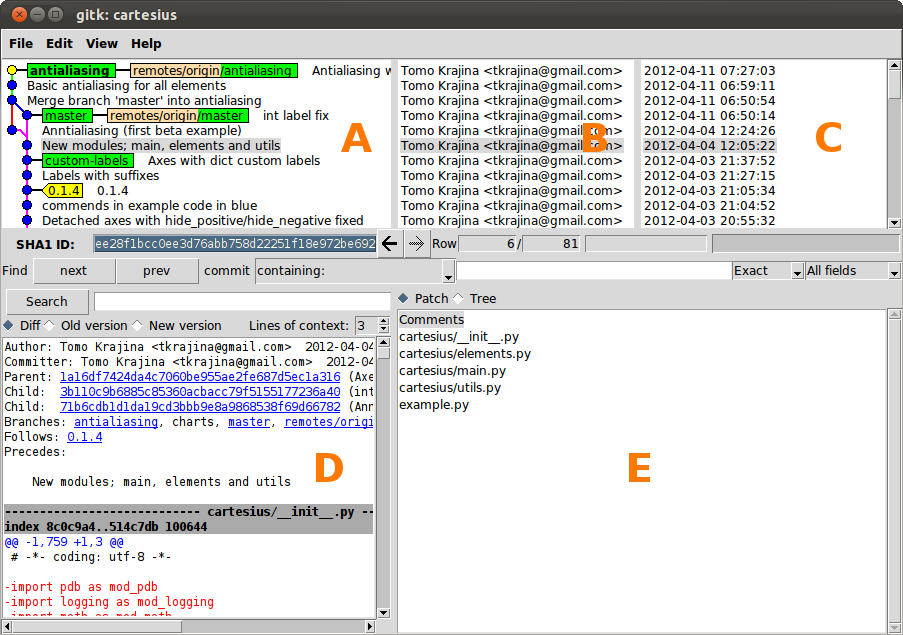
\includegraphics[width=14cm]{images/gitk.png}

Prikazani dijelovi su, redom s lijeva na desno od gore prema dolje:

\begin{itemize}
	\item grafički prikaz povijesti grane i \emph{commit}ova iz drugih grana koji su imali veze s tom granom (bilo zbog grananja, \emph{merge}anja ili \emph{cherry-pick} \emph{merge}),
	\item spisak ljudi koji su \emph{commit}ali,
	\item datum i vrijeme, 
	\item pregled svih izmjena,
	\item pregled datoteka koje su izmijenjene.
\end{itemize}

Kad odaberete \emph{commit} dobiti ćete sve izmjene i datoteke koje su sudjelovale.
Kad odaberete na datoteku, \verb+gitk+ će u dijelu sa izmjenama "skočiti" na izmjene koje su se dogodile na toj datoteci.

Gitk vam može i pregledati povijest samo do nekog \emph{commit}a u povijesti:

\gitoutputcommand{gitk HEAD\textasciitilde{}10}

\dots{}ili:

\gitoutputcommand{gitk 974ef0ad8351ba7b4d402b8ae3942c96d667e199}

\dots{}ili određene grane:

\gitoutputcommand{gitk testna-grana}

Kao i \verb+git gui+, tako i \verb+gitk+ na prvi pogled možda baš i nije jako intuitivan.
No, brz je i praktičan za rad kad se naučite na njegovo grafičko sučelje.

%\section*{}
%\addcontentsline{toc}{section}{}
